\def\currentRootFolder{chapter/statisticalMethods}
\def\currentFigureFolder{\currentRootFolder/fig}
\newcommand{\dataVec}{\vect{x}}
\newcommand{\paramVec}{\vect{\theta}}
\newcommand{\paramVecShared}{\vect{\theta}_\mathrm{s}}

\newcommand{\nuisanceParamVec}{\vect{\pi}}
\newcommand{\profLikelihood}{L_\mathrm{p}}

\makeatletter
\newcommand{\@giventhatstar}[2]{\left(#1\;\middle|\;#2\right)}
\newcommand{\@giventhatnostar}[3][]{#1(#2\;#1|\;#3#1)}
\newcommand{\giventhat}{\@ifstar\@giventhatstar\@giventhatnostar}
\makeatother

\newcommand{\Nobsi}{N_{\mathrm{obs,}i}}
\newcommand{\Ntheoi}{N_{\mathrm{theo,}i}}

\newcommand{\totUncert}{\sigma(\nuMass^2)}
\newcommand{\statUncert}{\sigma_\mathrm{stat}(\nuMass^2)}
\newcommand{\sysUncert}{\sigma_\mathrm{sys}(\nuMass^2)}
\newcommand{\statUncertTDR}{\sigma_\mathrm{stat}^\mathrm{TDR}(\nuMass^2)}
\newcommand{\sysUncertTDR}{\sigma_\mathrm{sys}^\mathrm{TDR}(\nuMass^2)}



\newacronym{mle}{MLE}{maximum likelihood estimator}
\chapter{Statistical Methods and Neutrino Mass Inference at KATRIN}
\label{sec:statMethods}
The best estimator for the neutrino mass alongside with an uncertainty or an upper limit will be retrieved by comparing the output of the KATRIN measurement with theoretical predictions within the process of parameter inference. This chapter reviews a selection of statistical approaches suitable in relation to the KATRIN experiment.

Section~\ref{sec:statMethodsMLE} outlines the principle of the \gls{mle}. Section~\ref{sec:statMethodsKATRINLikelihood} relates the principle of the \gls{mle} to a KATRIN measurement and neutrino mass inference. Section~\ref{sec:statMethodsStandardFit} introduces the formalism of a nominal neutrino mass fit at KATRIN. Section~\ref{sec:statMethodsUncertaintyIntervals} reviews the concept of uncertainty intervals and how confidence intervals can be extracted from the likelihood. Section~\ref{sec:statMethodsKaFitSSC} introduces the software framework that was used for simulated neutrino mass inference within this thesis. And section~\ref{sec:statMethodsKatrinSensitivity} explains the origin of the often quoted $\SI{200}{meV}$ (\SI{90}{\percent} C.L.) KATRIN sensitivity.

\section{Maximum Likelihood Estimation}
\label{sec:statMethodsMLE}
The likelihood is the probability of a measurement outcome given a hypothesis. A hypothesis depending on a parameter vector $\paramVec$ is called a composite hypothesis. A measurement outcome can be quantified by a vector of observed values $\dataVec$. The probability $P$ of $\dataVec$ given a hypothesis in dependence of $\paramVec$ is called the likelihood function~\cite{ReviewOfParticlePhysics}
\begin{equation}
	L(\paramVec) = P\giventhat{\dataVec}{\paramVec}
	\fullstop
\end{equation}
If $p$ denotes the probability of the independent and identically distributed observed values $x_i$ in $\dataVec$, then the likelihood function can be written as a product~\cite{ReviewOfParticlePhysics}
\begin{equation}
	L(\paramVec) = \prod_{i} p\giventhat{x_i}{\paramVec}
	\fullstop
\end{equation}
The parameter vector $\hat{\paramVec}$ that maximizes the likelihood function is called the \glsentryfull{mle} for the true values of $\paramVec$.

\section{The Likelihood of a KATRIN Measurement}
\label{sec:statMethodsKATRINLikelihood}
The \gls{mle}-method can be applied to a KATRIN measurement as follows: The data vector is given by a set of $n$ electron counts $\left\{\Nobsi\right\}$ measured at retarding energies $\left\{qU_i\right\}$. The following hypothesis can be formulated:

\begin{quote}
	$\left\{\Nobsi\right\}$ follow a Poisson distribution with predicted, expected electron counts $\left\{\Ntheoi(\paramVec)\right\}$ as per equation \eqref{eq:intSpecModelDetectorCounts}~\cite{Kleesiek2014}.
\end{quote}
The parameters $\paramVec$ of this composite hypothesis are discussed in the subsequent section~\ref{sec:statMethodsStandardFit}. For sufficiently high counts ($\gtrsim25$~\cite{Kleesiek2019}), the Poisson distribution can be approximated by a Gaussian distribution $\mathcal{N}(x,\mu, \sigma)$ with mean $\mu=\Ntheoi(\paramVec)$ and standard deviation $\sigma=\sqrt{\Nobsi}$. The likelihood function then reads~\cite{Kleesiek2014}
\begin{equation}
	\label{eq:KATRINlikelihood}
	L(\paramVec) = \prod_{i}^{n} \mathcal{N}\left(
		x=\Nobsi,
		\mu=\Ntheoi(\paramVec),
		\sigma=\sqrt{\Nobsi}
	\right)
	\fullstop
\end{equation}
Commonly, instead of maximizing the likelihood function, its negative logarithm is minimized and a factor 2 is introduced~\cite{ReviewOfParticlePhysics}. This yields
\begin{equation}
	\label{eq:statMethodsKatrinChi2}
	-2\ln L(\paramVec) = \chi^2(\paramVec) = \sum_i^n
		\left( 
			\frac{\Nobsi-\Ntheoi(\paramVec)}{\sqrt{\Nobsi}}
		\right)^2
		 + \mathrm{constants}
		\fullstop
\end{equation}
The minimization of equation~\eqref{eq:statMethodsKatrinChi2} yields the \gls{mle} estimator $\hat{\paramVec}$ for $\paramVec$.

Equation~\eqref{eq:statMethodsKatrinChi2} is a sum of $n$ random variables following a standard normal distribution. Hence, evaluated at the \gls{mle}, this chi-square expression $\chi^2(\hat{\paramVec})$ follows the so-called Pearson's chi-square statistic with $n-\mathrm{dim}(\paramVec)$ degrees of freedom. Accordingly, the value $\chi^2(\hat{\paramVec})$ is a measure for the goodness-of-fit~\cite{ReviewOfParticlePhysics}. In other words, $\chi^2(\hat{\paramVec})$ is a measure on how likely the data is under the hypothesis stated at the beginning of this section and can be used to reject it if the data is ``not a good fit for the hypothesis''.

In conclusion, equation~\eqref{eq:statMethodsKatrinChi2} can be used for parameter inference via the maximum likelihood method at KATRIN.

\section{A Nominal KATRIN Neutrino-Mass Fit}
\label{sec:statMethodsStandardFit}
With regard to a KATRIN neutrino mass measurement, the parameter of interest in the parameter vector $\paramVec$ is the squared neutrino mass $m_\nu^2$. Furthermore, $\paramVec$ typically comprises: the endpoint of the tritium-$\upbeta$ spectrum $E_0$ (eq.~\ref{eq:intSpecModelDiffSpecNeutrinoEnergy}), an overall normalization factor for the $\upbeta$-electron counts $\sigAmp$ (eq.~\ref{eq:intSpecModelDetectorCounts}) and the background rate $\bgRate$ (eq.~\ref{eq:intSpecModelDetectorCounts})~\cite{Kleesiek2014,Angrik:2005ep}. Hence, in order to infer the squared neutrino mass, the following four-dimensional likelihood has to be minimized:
\begin{equation}
\label{eq:statMethodsNominalKatrinChi2}
\chi^2(\paramVec) = \sum_i^n
\left( 
\frac{\Nobsi-\Ntheoi(\nuMass^2,E_0,\sigAmp, \bgRate)}{\sqrt{\Nobsi}}
\right)^2
\fullstop
\end{equation}
Applying this procedure with simulated data enables the determination of KATRIN's sensitivity to the neutrino mass (see subsequent section~\ref{sec:statMethodsKatrinSensitivity}).

\section{Uncertainty Intervals}
\label{sec:statMethodsUncertaintyIntervals}
The presented maximum likelihood method (section~\ref{sec:statMethodsMLE}) provides point estimates $\hat{\paramVec}$. However, additional information can be provided by interval estimates. There are two main approaches to statistical inference, which may be called Bayesian and frequentist~\cite{ReviewOfParticlePhysics}. They differ in their interpretation of probability, which becomes especially evident by the interval estimates associated with the two approaches: Credible and confidence intervals. The following two sections~\ref{sec:statMethodsUncertaintyIntervalsCredible} and~\ref{sec:statMethodsUncertaintyIntervalsConfidence} explain the matter in more detail.

\subsection{Bayesian Credible Intervals}
\label{sec:statMethodsUncertaintyIntervalsCredible}
The likelihood $L\giventhat{\dataVec}{\paramVec}$ is a probability distribution for the data $\dataVec$ given the parameters $\paramVec$. It can be transformed into a probability density for the parameters $\paramVec$ by multiplication with a prior distribution $\pi(\paramVec)$ and normalization to one using Bayes' theorem. The result is the posterior distribution~\cite{ReviewOfParticlePhysics}
\begin{equation}
\label{eq:statMethodsPosterior}
	P\giventhat{\paramVec}{\dataVec} = 
		\frac{
			L\giventhat{\dataVec}{\paramVec}\cdot\pi(\paramVec)
		}{
			\int L\giventhat{\dataVec}{\paramVec^\prime}\cdot\pi(\paramVec^\prime) \d\paramVec^\prime
		}
	\fullstop
\end{equation}
Bayesian statistics provide no fundamental rule for obtaining the prior probability~\cite{ReviewOfParticlePhysics}. This freedom of choice may reflect subjectivity and thus causes controversy. 

The posterior is a multi-dimensional probability distribution. With regard to the KATRIN experiment, there is one parameter of interest, namely, the squared neutrino mass $\nuMass^2$. The other dimensions in the parameter space, denoted by $\vect{\nu}$, can be marginalized~\cite{ReviewOfParticlePhysics}
\begin{equation}
	p\giventhat{\nuMass^2}{\dataVec} = \int P\giventhat{\paramVec\equiv(\nuMass^2,\vect{\nu})}{\dataVec} \d \vect{\nu}
	\fullstop
\end{equation}
This yields a one-dimensional probability distribution for the squared neutrino mass, from which a credible interval can be extracted.

The prior $\pi(\paramVec\equiv(\nuMass^2,\vect{\nu}))$ can be chosen such that it vanishes for $\nuMass^2<0$. Equation~\eqref{eq:statMethodsPosterior} shows that then also the posterior vanishes for $\nuMass^2<0$ independently of the likelihood. In other words, the likelihood does not have to be evaluated for negative, unphysical squared neutrino masses.



\subsection{Frequentist Confidence Intervals}
\label{sec:statMethodsUncertaintyIntervalsConfidence}
In chapter~\ref{sec:katrinEloss} of this thesis, a sensitivity study is presented that is based on the idea of confidence intervals. Therefore, in this section, the topic is treated in some detail. First, definitions are given for the terms ``confidence interval'', ``coverage probability'' and ``confidence level''. Then, it is explained, how confidence intervals can be constructed using the likelihood. 

The unqualified phrase ``confidence interval''~\cite{ReviewOfParticlePhysics} refers to frequentist intervals obtained with a procedure introduced by Neyman~\cite{Neyman1937} (this Neyman construction is not shown in this thesis, instead another construction is given below, that finds application in chapter~\ref{sec:katrinEloss}). Confidence intervals are given with reference to a parameter $\theta$ that is to be estimated from the data. Within the Neyman construction, the boundary of a confidence interval is given by a function of the data~\cite{ReviewOfParticlePhysics}. This means, the boundary of a confidence interval would fluctuate if one were to repeat the experiment many times (because each time, the obtained data would be different). An ensemble of confidence intervals would be obtained. The coverage probability $\alpha$ refers to the fraction of confidence intervals in such a hypothetical ensemble that contains the true parameter value of $\theta$~\cite{ReviewOfParticlePhysics}. If, in the limit of a large ensemble size, the confidence intervals cover the true parameter value at least a fraction of $\alpha$ times, the confidence interval obtained from only one data set is understood to have a confidence level of $\alpha$~\cite{ReviewOfParticlePhysics}. (An illustration of this abstract definition is developed throughout the subsequent section~\ref{sec:katrinElossStatistics} in the context of a sensitivity study. Furthermore, a simulated ensemble of confidence intervals with the corresponding coverage probability is shown in figure~\ref{fig:katrinElossResultsCoverage}.)

In a practical context, a prescription is required on how to construct confidence intervals of an eligible confidence level. The Neyman construction~\cite{Neyman1937}, as mentioned, or the unified approach by Feldman and Cousins~\cite{Feldman1998} are such prescriptions. The unified approach is based on the likelihood ratio. An ordering principle enables the construction of a confidence interval that may either represent an upper limit or and upper as well as a lower limit. How a confidence interval can be obtained via the likelihood ratio is shown below. However, a so-called classical confidence interval is constructed that always has an upper and a lower limit and is centrally located around the \gls{mle}. 

\paragraph{Construction of a Classical Confidence Interval using the Likelihood Ratio}
\begin{figure}
	\centering
	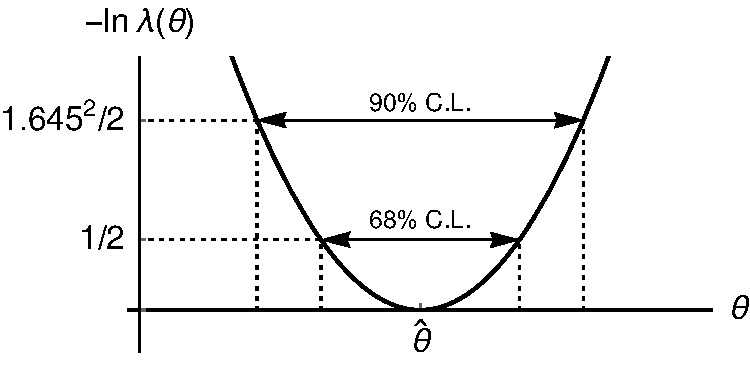
\includegraphics[width=\textwidth]{\currentFigureFolder/confidenceIntervalIllustration.pdf}
	\xcaption{Illustration of a confidence interval obtained via the likelihood ratio}{Illustration of a confidence interval obtained via the likelihood ratio.}{The graph illustrates equation~\eqref{eq:statMethodsLikelihoodRatio} on how to extract a confidence interval from a one-dimensional likelihood of Gaussian shape. The negative logarithm of the likelihood ratio (eq.~\ref{eq:statMethodsLikelihoodRatio}) is shown, which is zero at the \gls{mle} $\hat{\paramVec}$ and increases in $s^2/2$-steps corresponding to confidence intervals of $s$-$\sigma$ C.L. (also refer to the main text).}
	\label{fig:statMethodsConfidenceContour}
\end{figure}
In this paragraph, the construction of a confidence region is discussed, which is the multidimensional generalization of a confidence interval for the case that the likelihood depends on more than one parameter (which is the case for the KATRIN likelihood). A method to construct a confidence region is to consider a test of the hypothesis that the parameter values $\paramVec$ have the true values $\paramVec_\mathrm{T}$~\cite{ReviewOfParticlePhysics}. All parameter values $\paramVec$ are excluded from the confidence region of confidence level $\alpha$ that are rejected by a test of size $\alpha$~\cite{ReviewOfParticlePhysics}. A possible test statistic for $\paramVec$ is the likelihood ratio of the likelihood at the \gls{mle} $\hat{\paramVec}$ and $\paramVec$~\cite{ReviewOfParticlePhysics}
\begin{equation}
	\label{eq:statMethodsLikelihoodRatio}
	\lambda(\paramVec) =
	\frac{L(\paramVec)}{L(\hat{\paramVec})}
	\fullstop
\end{equation}
If the likelihood follows the form of a multivariate Gaussian distribution in $\paramVec$, then the above test statistic~\eqref{eq:statMethodsLikelihoodRatio} can be evaluated and the hyper surface defined by
\begin{equation}
	\label{eq:statMethodsConfidenceContour}
	-\ln \lambda(\paramVec) = \frac{s^2}{2}
\end{equation}
approximately encloses a $s$-$\sigma$ confidence region for $\paramVec$~\cite{ReviewOfParticlePhysics}. Here, $s$-$\sigma$ denotes the corresponding quantile of a Gaussian distribution (for example, $s\approx1$ for \SI{68}{\percent} C.L.~or $s\approx1.645$ for \SI{90}{\percent} C.L.). 

Equation~\eqref{eq:statMethodsConfidenceContour} is illustrated in figure~\ref{fig:statMethodsConfidenceContour} for the case that $\paramVec$ is one-dimensional. However, in a realistic scenario, $\paramVec$ comprises more than one dimension (at least four in a nominal KATRIN neutrino mass fit, see previous section~\ref{sec:statMethodsStandardFit}). Extracting a confidence interval only for the squared neutrino mass requires further steps. The introduction of a formalism (profile-likelihood method) that handles the additional dimensions of the nuisance parameters is postponed to the subsequent section~\ref{sec:katrinElossStatisticsProfileLikelihood} where it is presented in the context of a practical example.

\paragraph{Negative Squared Neutrino Masses}
It should be noted, that the extraction of confidence intervals from the KATRIN likelihood requires its extrapolation to nonphysical, negative squared neutrino masses - a complication that can be avoided when using Bayesian methods as described in the previous section~\ref{sec:statMethodsUncertaintyIntervalsCredible}. In this thesis, the strategy proposed by~\cite{WEINHEIMER1993} (and implemented in the scope of \cite{Kleesiek2014}) is used and the formula for the phase-space factor of the neutrino in the differential $\upbeta$ decay rate~\eqref{eq:intSpecModelDiffSpec} is adapted for negative squared neutrino masses
\begin{equation}
\begin{split}
&\sum_{f} 
P_f \cdot 
\epsilon_f \cdot 
\sqrt{\epsilon_f^2-\nuMass^2} \cdot 
\thetaFunc(\epsilon_f-\nuMass)
\rightarrow
\sum_{f} 
P_f \cdot 
(
	\epsilon_f + 
	m_\nu^\prime\cdot 
	\euler^{-(\frac{\epsilon_f}{m_\nu^\prime}+1)}	
) \cdot 
\sqrt{\epsilon_f^2-\nuMass^2} \\
&\text{ with } m_\nu^\prime = \mu \cdot \sqrt{-\nuMass^2}
\end{split}
\fullstop
\end{equation}
The factor $\mu$ can be adapted in order to provide an approximately symmetric log-likelihood function around $\nuMass^2=0$. In this thesis, $\mu=0.717$ was used. An approximate symmetry was achieved (see for example table~\ref{tab:katrinElossModelResultsAsimov} and figure~\ref{fig:katrinElossResultsProfileLikelihood}). In order to achieve a perfect symmetry, the factor might need adaption depending on the actual study and the model of the detector counts as per equation~\eqref{eq:intSpecModelDetectorCounts} (for example, \cite{WEINHEIMER1993} suggests $\mu=0.76$).

In conclusion, in this section, an outline of confidence intervals has been given. It has also been shown how a confidence region can be constructed using the KATRIN likelihood. 

\section{The KaFit and SSC Software Frameworks}
\label{sec:statMethodsKaFitSSC}
With respect to neutrino mass inference at KATRIN, two components have been presented: a model for a KATRIN neutrino mass measurement in chapter~\ref{sec:intSpecModel} and a statistical framework for parameter inference within the current chapter~\ref{sec:statMethods}.

The two components are implemented within two modules of the \gls{kasper}~\cite{Kasper}:\mynobreakpar
\begin{enumerate}
	\item The \textbf{\glsentryfull{ssc}}~\cite{SSC} module implements the formulas as per chapter~\ref{sec:intSpecModel}. Additionally, it also includes aspects beyond the given description, for example the gas dynamics within the \gls{wgts}. It is based on several previous works, such as~\cite{Hoetzel2012, Groh2015, Kleesiek2019, Kaefer2012, Heizmann2018, Kuckert2018}.
	\item The \textbf{\gls{kafit}}~\cite{KaFit} module translates the $\upbeta$ spectrum calculated by \glsentryshort{ssc} into predicted detector counts~\cite{Kleesiek2014}. Furthermore, \gls{kafit} implements several statistic tools tailored to the KATRIN experiment, one of which is the extraction of confidence intervals according to the profile-likelihood method (see subsequent section~\ref{sec:katrinElossStatisticsProfileLikelihood}), which is of importance in the scope of this thesis. The actual minimization and profiling are done by the interfaced MINUIT2~\cite{James1998} and MINOS package from the ROOT~\cite{ANTCHEVA2009} analysis framework.
\end{enumerate}

Both modules were used and extended to allow for the analysis done in the scope of this thesis as is explained in the subsequent chapters~\ref{sec:eDepScatCrossSec} and~\ref{sec:katrinEloss}.

\section{KATRIN's Sensitivity to the Neutrino Mass}
\label{sec:statMethodsKatrinSensitivity}
This section explains the origin of the often quoted KATRIN design sensitivity to the neutrino mass of $\SI{200}{meV}$\,(\SI{90}{\percent} C.L.). First, a definition of the sensitivity is given in section~\ref{sec:statMethodsSensitivtyDef}. Subsequently, section~\ref{sec:statMethodsSensitivtyFromEnsemble} and~\ref{sec:statMethodsSensitivtyFromProileLikelihood} show how this definition was applied by different works to deduce KATRIN's sensitivity.

\subsection{Definition and Construction of KATRIN's Sensitivity}
\label{sec:statMethodsSensitivtyDef}
\begin{figure}
	\centering
	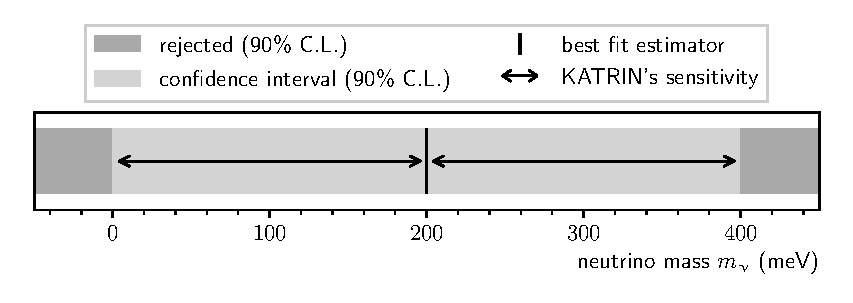
\includegraphics[width=\textwidth]{\currentFigureFolder/sensitivityIllustration.pdf}
	\xcaption{Illustration of KATRIN's sensitivity to the neutrino mass}{Illustration of KATRIN's sensitivity to the neutrino mass.}{The graph illustrates KATRIN's sensitivity of~\SI{200}{meV}~\cite{Angrik:2005ep} as per equation~\eqref{eq:statMethodsSensitivity}. It shows a hypothetical measurement of the neutrino mass that yields a symmetric confidence interval \mbox{(\SI{90}{\percent} C.L.)} centrally located around the best fit estimator. If such a classical confidence interval is constructed, KATRIN can reject the null hypothesis of a vanishing neutrino mass at \mbox{\SI{90}{\percent} C.L.} if it estimates a neutrino mass of at least~\SI{200}{meV}.}
	\label{fig:statMethodsSensitivity}
\end{figure}

KATRIN's sensitivity can be understood as half the width of a symmetric and central confidence interval (\SI{90}{\percent} C.L.) for the neutrino mass obtained from a KATRIN neutrino mass measurement. As such, it can be constructed from a 1-$\sigma$ uncertainty $\totUncert$ on the squared neutrino mass~\cite{Angrik:2005ep}
\begin{equation}
\label{eq:statMethodsSensitivity}
S_{\nuMass}(\SI{90}{\percent}) = \sqrt{1.645\cdot\totUncert}
\comma
\end{equation}
where the factor 1.645 translates the $\SI{68.3}{\percent}$ interval into a $\SI{90}{\percent}$ interval in the case of Gaussian uncertainties.

In other words, KATRIN's sensitivity to the neutrino mass can be understood as the minimal neutrino mass that has to be inferred from a KATRIN neutrino mass measurement to exclude the null hypothesis of a vanishing neutrino mass~\cite{Kleesiek2014} when constructing a classical confidence interval (\SI{90}{\percent} C.L.). Figure~\ref{fig:statMethodsSensitivity} illustrates this statement.

For a more comprehensive picture, where not only a classical interval is considered, but also the unified approach according to Feldmann and Cousins as well as Bayesian statistics, the reader is referred to~\cite{Kleesiek2019}. These techniques also allow to interpret KATRIN's sensitivity as an upper limit that can be established for the neutrino mass if a vanishing neutrino mass is measured.

\subsection{Sensitivity from Simulated Ensembles}
\label{sec:statMethodsSensitivtyFromEnsemble}
In the KATRIN Design Report, the sensitivity to the neutrino mass was evaluated using ensemble tests. An ensemble of many KATRIN measurements was simulated (see section~\ref{sec:intSpecModelNuMassMeasurement} on how such a simulation can be conducted) with a true neutrino mass of \SI{0}{eV}. From each simulated measurement, the squared neutrino mass was inferred in a standard KATRIN four-parameter fit (see section~\ref{sec:statMethodsStandardFit}). The central 1-$\sigma$ interval of the obtained ensemble of squared neutrino masses was taken as the statistical uncertainty on the squared neutrino mass~\cite{Angrik:2005ep}
\begin{equation}
	\statUncertTDR = \SI{0.018}{eV^2}
	\fullstop
\end{equation}
The systematic uncertainty was estimated to be approximately \SI{0.01}{eV}. Due to the early stage of the experiment the systematic uncertainty was conservatively enlarged to a systematic budget at approximately the same scale as the statistical uncertainty~\cite{Angrik:2005ep}
\begin{equation}
	\label{eq:statMethodsSensitivtyFromEnsembleTDRSysBudget}
	\sysUncertTDR = \SI{0.017}{eV^2}
	\fullstop
\end{equation}
Adding the statistic and systematic uncertainty quadratically and applying the definition~\eqref{eq:statMethodsSensitivity} yields KATRIN's design sensitivity~\cite{Angrik:2005ep}
\begin{equation}
	\label{eq:statMethodsSensitivityDesignReport}
	S_{\nuMass}^{\mathrm{TDR}}(\SI{90}{\percent}) = 
	\sqrt{1.645\cdot
		\sqrt{
		\statUncertTDR^2+\sysUncertTDR^2
	}}
	\approx \SI{200}{meV}
	\fullstop
\end{equation}
The corresponding investigations were redone in the scope of several works. Table~\ref{tab:statMethodsSensitivityFromEnsembleTests} lists selected results.
\begin{table}[tb]
	\centering
	\xcaption{KATRIN's sensitivity to the neutrino mass from ensemble tests}{KATRIN's sensitivity to the neutrino mass from ensemble tests.}{The table lists KATRIN's sensitivity~$S_{\nuMass}(\SI{90}{\percent})$ as defined by equation~\eqref{eq:statMethodsSensitivity}. Several works reevaluated the statistical uncertainty according to experimental and theoretical progress. For each reevaluation, a systematic uncertainty of $\sysUncert = \SI{0.017}{eV^2}$ was assumed. A value derived from an ensemble test is a random variable. Corresponding widths of the obtained distributions are reprinted if they were originally stated.}
	\begin{tabular}{lrlr}
		\toprule
		\makecell[t]{$\statUncert$ (\SI{}{eV^2})} & 
		\makecell[t]{$S_{\nuMass}(\SI{90}{\percent})$ (\SI{}{meV})} & 
		\makecell[t]{comment} &
		\makecell[t]{reference}
		\\
		\hline
		0.018 & 200 & design value & \cite{Angrik:2005ep} \\
		$0.0165\pm0.0001$ & 198 & updated $\upbeta$-spectrum calculation & \cite{Hoetzel2012} \\
		$0.0162\pm0.0001$ & 197 & further updated $\upbeta$-spectrum calculation & \cite{Kleesiek2014} \\
		0.01490 & 193 & optimized \gls{mtd} & \cite{Kleesiek2014} \\
		\bottomrule
	\end{tabular}
	\label{tab:statMethodsSensitivityFromEnsembleTests}
\end{table}
\subsection{Sensitivity from  the Profile-Likelihood Method}
\label{sec:statMethodsSensitivtyFromProileLikelihood}
The approach shown above via ensemble testing yields an ensemble respectively a distribution of estimated squared neutrino masses. The sensitivity is then derived from this ensemble. Instead of using an ensemble of inferred squared neutrino masses, also an ensemble of confidence intervals may be used. This approach is explained in chapter~\ref{sec:katrinEloss}. In order to deduce a confidence interval from a single measurement, the profile-likelihood method (see subsequent section~\ref{sec:katrinElossStatisticsProfileLikelihood}) may be used, which finds application in the scope of this thesis.

For comparison, previous results from~\cite{Kleesiek2014} based on the profile-likelihood method are shortly reviewed here: Two uncertainties were obtained for two different~\gls{mtd}s in a KATRIN standard four-parameter fit (see section~\ref{sec:statMethodsStandardFit}). The first \gls{mtd} had been specially optimized with regard to KATRIN's sensitivity and the resulting statistical uncertainty is $\statUncert=\SI{0.01494}{eV^2}$. For the second result, the nominal \gls{mtd} from the KATRIN Design Report (see section~\ref{sec:intSpecModelMTD}) was used. The corresponding profile likelihood was plotted and $\statUncert$ can be extracted to be between \SI{0.0155}{} and \SI{0.0165}{eV^2}. Both results are in agreement with the results from ensemble tests (see~\cite{Kleesiek2014} in table~\ref{tab:statMethodsSensitivityFromEnsembleTests}).